\section{Analysis of the cylindrical detector system\label{sec-anacds}}
The cylindrical detector system (CDS) is mainly used for the reconstruction of reaction vertex to derive the missing mass spectrum of the $^3$He$(K^-,n)$ reaction. However, more detailed analysis, such as particle identification and momentum reconstruction, was carried out to check the performance of whole spectrometer system. %In this section, the analysis and calibration method of the CDS presented. %Later in Sec, \ref{} the whole system performance will be checked in combination with the forward TOF counters.

An analysis procedure of the CDS is as follows:
\begin{enumerate}
\item Track finding in the CDC.
\item Search for associated hits on the IH and the CDH for each CDC track.
\item Reconstruct a vertex point with a beam track, and calculate mass-square of the CDC tracks.
\item Re-fit the CDC tracks after applying fine corrections on the CDC hits, and re-calculate the mass-square.
\item Identify particle species of each CDC track with a momentum and a re-calculated mass-square.
\item Re-calculate the vertex point, and obtain the momentum three-vector of each CDC track at the vertex.
\end{enumerate}

\subsection{Tracking with the CDC} 
A trajectory of a charged particle in a magnetic field can be expressed with a helix if the field is uniform. 
To check whether the helix can describe a charged track in the CDS,  a simulation data was generated in the calculated solenoid field by the TOSCA code. The simulation data was analyzed assuming the uniform field, and we confirmed that the helix can describe the charged particle tracks with a momentum precision better than 0.2\%. Therefore, the helix expression was employed for a CDC track.  
\subsubsection{Helix parametrization}
A helix at the CDC local coordinate can be parametrized as,%\cite{helix},
\begin{eqnarray*}
x(\phi) &=&d_\rho\cos\phi_0+\frac{1}{\rho}\left(\cos\phi_0-\cos(\phi_0+\phi)\right)\\
y(\phi) &=&d_\rho\sin\phi_0+\frac{1}{\rho}\left(\sin\phi_0-\sin(\phi_0+\phi)\right)\\
z(\phi) &=&d_z-\frac{1}{\rho}\tan\lambda\cdot\phi,
\end{eqnarray*}
where $d_\rho$ is the distance of the helix from pivotal point in the $xy$ plane, $\phi_0$ is the azimuthal angle to specify the pivotal point with respect to the helix center, $\rho$ is the inverse of the signed radius of the helix, $d_z$ is the distance of the helix from the pivotal point in the $z$ direction, and $\tan\lambda$ is the dip angle. The deflection angle $\phi$ is measured from the pivotal point, and specifies the position of the charged particle on the helical track. %The meanings of these parameters are depicted in Fig. \ref{fig-helix}.

The momentum of a charged particle is related to its helix parameters as,
\begin{eqnarray*}
{ \mathbf p} &=& \frac{cB}{\rho} \left( 
	\begin{array}{c}
	-\sin(\phi_0+\phi) \\	
	\cos(\phi_0+\phi) \\
	\tan\lambda
	\end{array}
	\right),
\end{eqnarray*}
where $c$ is the light velocity and $B$ is the strength of the magnetic field in the $z$ direction.

%\begin{figure}[]
%\begin{center}
%\includegraphics[width=\columnwidth]{./illustrator/helix.eps}
%\caption{}
%\label{fig-helix}
%\end{center}
%\end{figure}  

\subsubsection{TDC data conversion to the drift length}
A method to convert from a TDC channel to a drift time is the same as that for the beam line drift chambers described in Sec. 3.3.2. Relative time offset in each wire was adjusted in a similar way to the beam line chambers at first. For the conversion from a drift time to a drift length, a fifth order polynomial function was employed. The conversion function was iteratively adjusted by minimizing systematic shifts in the residuals as a function of the drift time. The residual was defined as subtracting the drift length from the shortest distance between the hit wire and the helix. A typical conversion function is shown in Fig. \ref{fig-cdcdtdl}. Note that additional fine tuning of the drift time was performed as described in Sec. 3.4.5.

\begin{figure}[]
\begin{center}
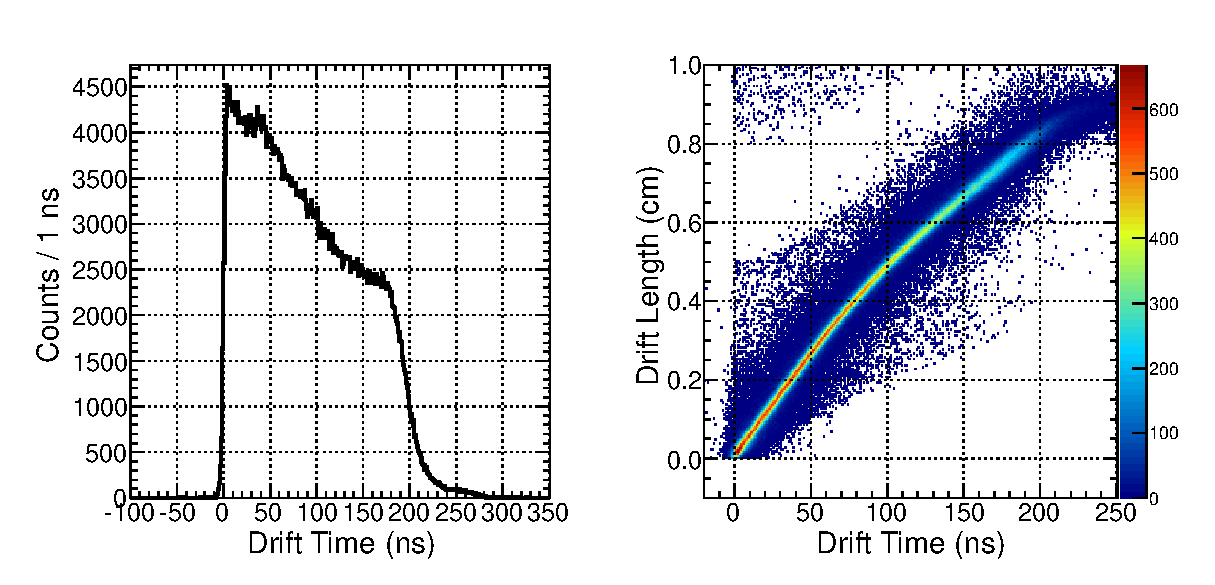
\includegraphics[width=\columnwidth]{./fig/cdcdtdl.eps}
\caption[Typical timing distribution and correlation between the drift time and the drift length of the CDC]{(left) Typical timing distribution of the CDC hit. (right) Typical correlation between the drift time and the drift length. }
\label{fig-cdcdtdl}
\end{center}
\end{figure}  

\subsubsection{Track finding and $\chi^2$ fitting}
First, track candidates were searched in $xy$ plane using only axial layers. A circle fitting was performed to determine the combination of hits in axial layers and to estimate helix parameters $d_\rho, \phi_0$, and $\rho$. %\cite{}. 
Then, associated hits in the stereo layers were searched in $z-\phi$ plane to estimate $d_z$ and $\tan\lambda$. Finally, full helix fitting was performed by using TMinuit to minimize the reduced-$\chi^2$, which was defined as,
\begin{eqnarray*}
\chi^2/ndf &=& \frac{1}{n-5}\sum_i^n \left(\frac{\delta_i-dl_i}{\sigma_i}\right)^2,
\end{eqnarray*}
where $n$ is the number of hits, $\delta_i$ is the shortest distance between the hit wire and the helix track, $dl_i$ is the drift length, and $\sigma_i$ is the spatial resolution of 180 $\mu m$ obtained in Sec. \ref{sec-cdcposres}. The resultant $\chi^2/ndf$ distribution is shown in Fig. \ref{fig-cdcchi} and tracks with $\chi^2/ndf < 30$ were defined as good tracks. Note that bad $\chi^2/ndf$ tracks were used in the multiplicity counting in the CDS.

A track was required to have at least one hit in each axial super layer. In addition, at least 5 hits in the stereo layers and at least 10 hits in total were required.
\begin{figure}[]
\begin{center}
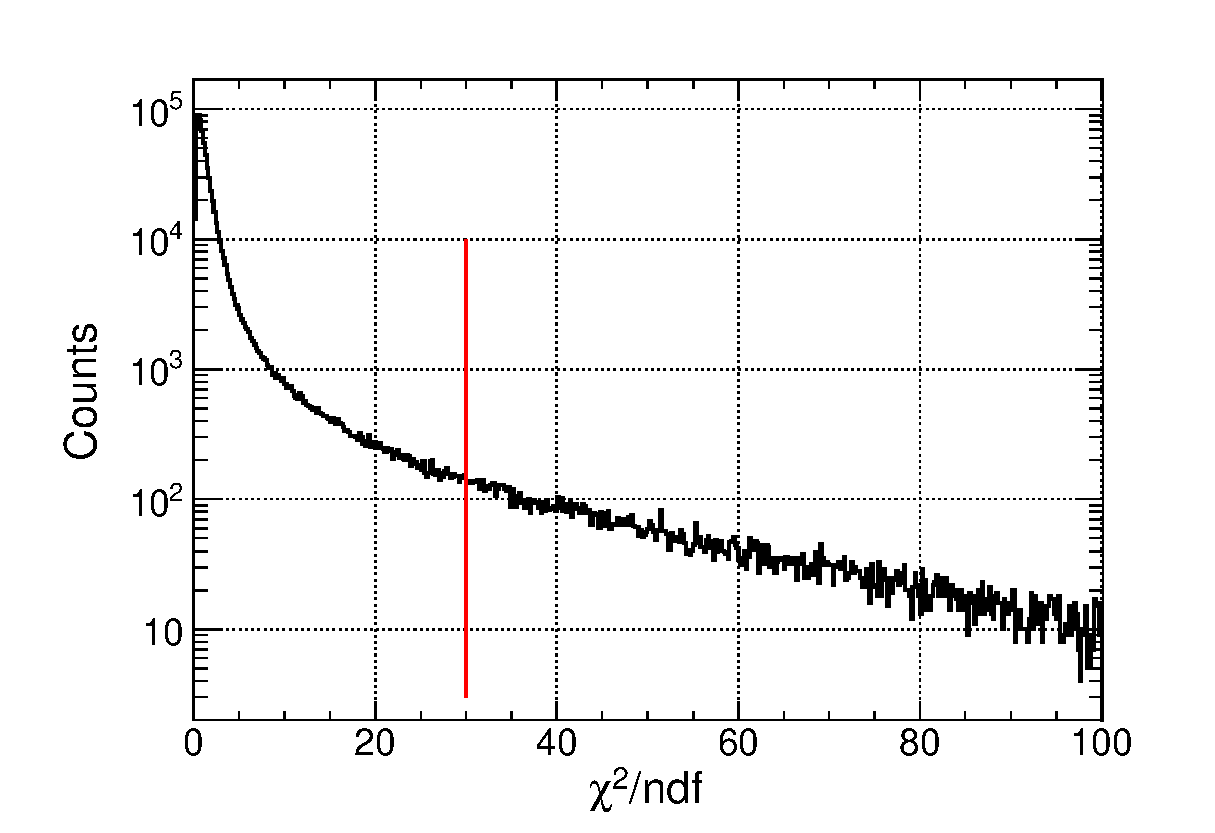
\includegraphics[width=12cm]{./fig/cdcchi.eps}
\caption[$\chi^2/ndf$ distribution in the CDC tracking. ]{$\chi^2/ndf$ distribution in the CDC tracking. Tracks with $\chi^2/ndf<$ 30 were accepted.}
\label{fig-cdcchi}
\end{center}
\end{figure}  

\subsection{Associated hit search in the IH and the CDH}
Once a CDC track was defined, associated hits in the IH and the CDH were determined by using extrapolated position of the track. Figure \ref{fig-cdchodo}(left) shows the azimuthal angle matching for the CDH at the inner radius of r = 544 mm when we obtained only one track in the CDC and one hit in the CDH. The matching efficiency is obtained to be better than 99\%.
In a general case, we also checked the matching at the outer radius of the CDH, r = 574 mm and accepted CDC tracks with multiple CDH hits. If multiple hits in the CDH was associated with one CDC track, the fastest timing segment was defined as the timing of the CDC track. 
For the IH, similar procedure was applied. Figure \ref{fig-cdchodo}(right) shows the azimuthal angle matching of the IH at the inner radius of r = 137 mm. The matching efficiency was $\sim$ 98\%.

\begin{figure}[]
\begin{center}
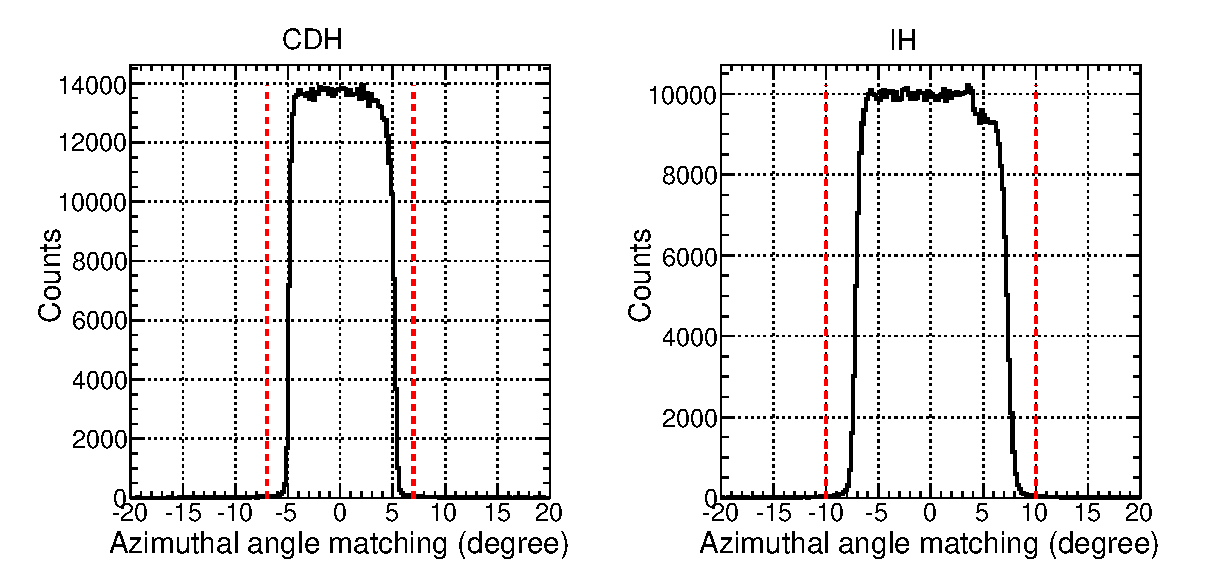
\includegraphics[width=\columnwidth]{./fig/cdc-ihcdhmatch.eps}
\caption[Azimuthal matching between a CDC track and a CDH/IH hit.]{Azimuthal matching of hits (left) on the CDH and (right) on the IH. Events between two red lines were accepted. The segment size corresponds to $\pm5^\circ$ and $\pm7.5^\circ$ for the CDH and the IH, respectively. }
\label{fig-cdchodo}
\end{center}
\end{figure}  

\subsection{Vertex reconstruction}
\subsubsection{Vertex with one CDC track}
With one CDC track, a candidate of the reaction-vertex point was obtained by the distance of the closest approach (DCA) using the BPC and the CDC track. The point on the BPC was defined as the candidate of the vertex as shown in Fig. \ref{fig-vertexreconstruction}(left). %Figure \ref{} is a schematic explanation.

\subsubsection{Vertex with two CDC tracks}
If an event had two or more CDC tracks, all possible pairs among them were examined to reconstruct a secondary vertex. The secondary vertex was defined as the center of DCA points of the two helical tracks. The momenta of the two tracks were recalculated at the secondary vertex with an energy loss correction, and the parent track was reconstructed. Then, the primary vertex, i.e. the reaction vertex, was obtained using the BPC track and the parent track and the DCA was used to selection of the vertex candidates as shown in Fig. \ref{fig-vertexreconstruction}(right).% as schematically shown in Fig. \ref{}.
\\

Among the vertex candidates obtained with one and two CDC tracks, the minimum DCA candidate was selected to be the reaction vertex. Figure \ref{fig-cdcdca}(left) shows the track multiplicity of the CDC with a neutron detection by the NC, and the Fig. \ref{fig-cdcdca} shows the difference of the DCA distribution due to the number of CDC tracks used to reconstruct the reaction vertex. In Fig. \ref{fig-cdcdca}(right), $\pi^+\pi^-$ pairs were analyzed and the difference of the vertex reconstruction method was found to be not so significant. Note that the displacement of the $z$-vertex position by 1 cm causes only $\sim$0.3 MeV/$c$ momentum deviation for a 1 GeV/$c$ neutron, which is much smaller than the precision of the current experiment. 


\begin{figure}[]
\begin{center}
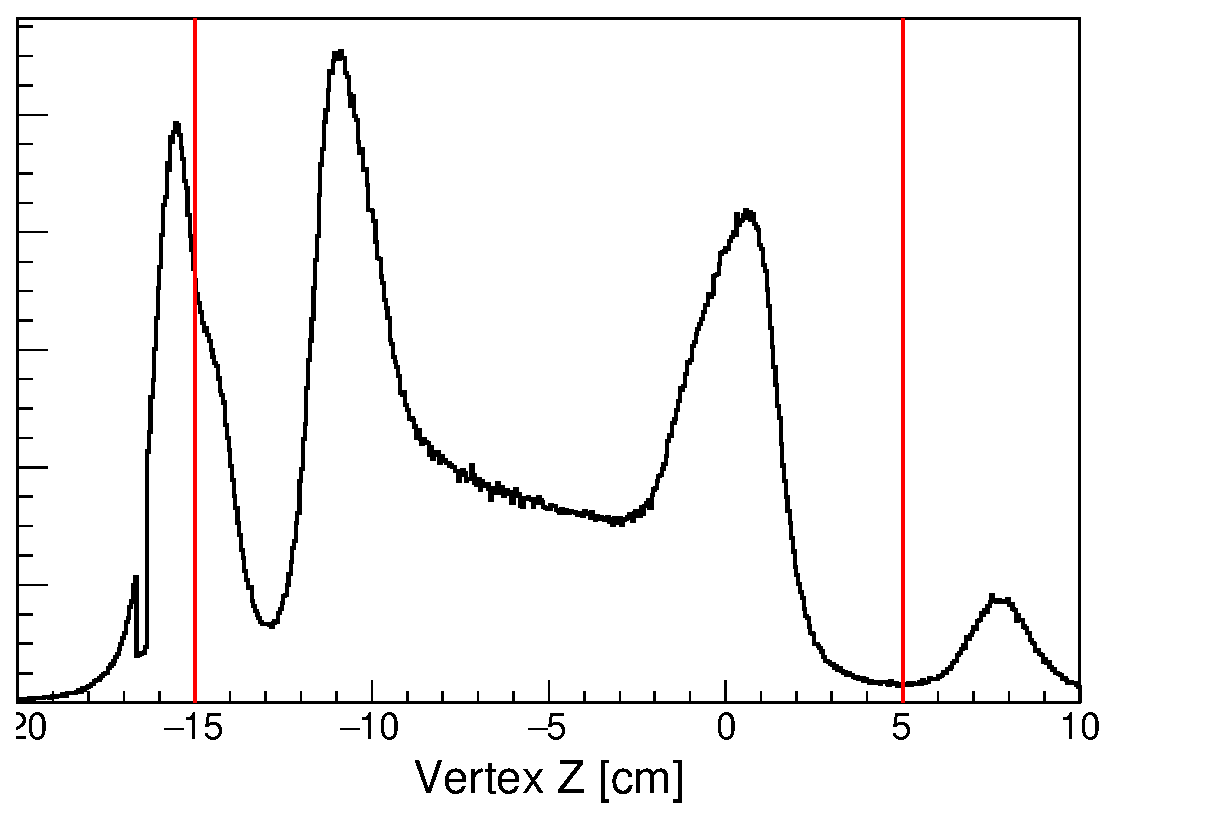
\includegraphics[width=\columnwidth]{./illustrator/vertex.eps}
\caption[Vertex reconstruction with BPC and CDC tracks.]{Vertex reconstruction with BPC and CDC tracks.}
\label{fig-vertexreconstruction}
\end{center}
\end{figure}  
\begin{figure}[]
\begin{center}
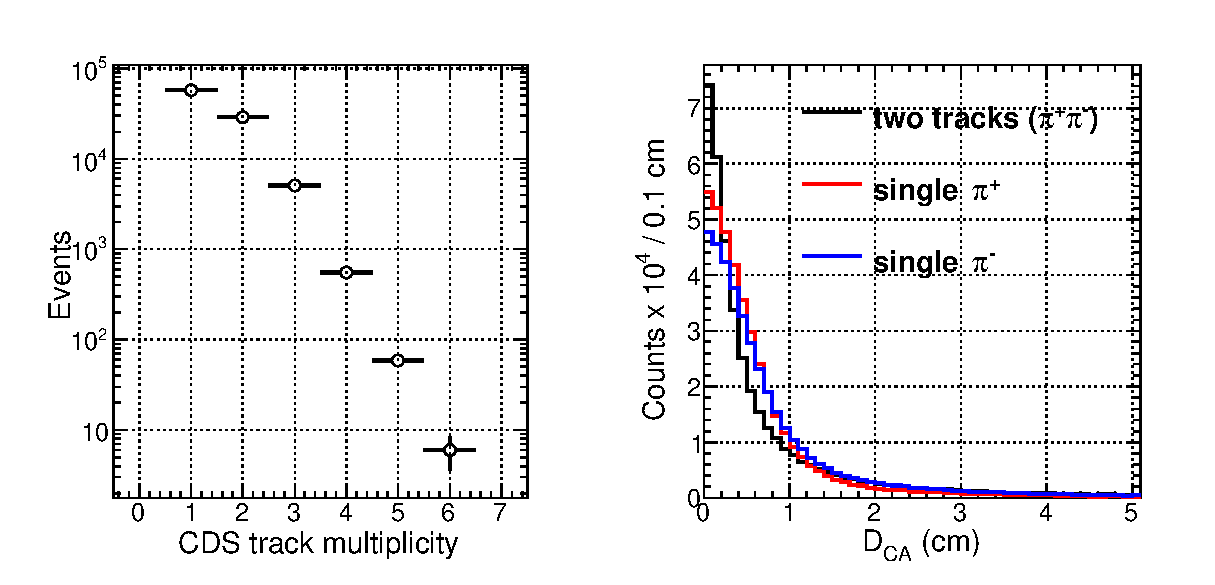
\includegraphics[width=\columnwidth]{./fig/cdc-mul.eps}
\caption[CDC track multiplicity and DCA distributions.]{(left) CDC track multiplicity. Neutron detection by the NC is requested. (right) DCA distributions of the events with $\pi^+\pi^-$ pairs detected by the CDS. The black, red, and blue histograms are obtained by using reconstructed parent track of the $\pi^+\pi^-$, the $\pi^-$ track, and the $\pi^+$ track, respectively.}
\label{fig-cdcdca}
\end{center}
\end{figure}  

\subsection{Particle identification}\label{sec-cdcpid}
A velocity $\beta$ and a mass $M$ of the CDC track can be calculated as,
\begin{eqnarray}
\beta &=& \frac{L_{CDC_{in}-CDH}}{\left((T_{CDH}-T_{T0}) - T^{calc}_{T0-vertex}- T^{calc}_{vertex-CDC_{in}} \right)\times c} \label{eq-cdsbeta}\\
%&&T^{calc}_{T0-vertex} = \frac{L_{T0-vertex}}{ \beta_{beam}c}\\
M^2&=&p^2\times \frac{1-\beta^2}{\beta^2},
\end{eqnarray}
where $\it{L_{CDC_{in}-CDH}}$ is the helical-track length between the entrance of CDC tracking volume at the radius of 15.1 cm and the CDH, $T_{CDH}$ - $T_{T0}$ is the measured flight time between the CDH and T0. $T^{calc}_{T0-vertex}$ and  $T^{calc}_{vertex-CDC_{in}}$ are calculated flight times between T0 and the vertex, and between the entrance of the CDC tracking volume and the CDH, respectively. Velocity and curvature changes by energy losses were taken into account. % as the detail is explained in Appendix \ref{}. 

The resultant distribution of the momentum versus the mass-square is shown in Fig. \ref{fig-cdspid2d}, where pions, kaons, protons and deuterons are clearly separated. In the current analysis, a particle identification is roughly done by using only the mass-square and the charge as shown in Fig. \ref{fig-cdspid1d}. Although the PID efficiencies are high at around 99\%, we did not remove electrons, positions and muons contaminated in the pion identification. Those contamination can be much suppressed if we used two dimensional particle identification in the mass-square and the momentum plane. 

\subsubsection{CDH calibration}
The velocity of the particle can be also calculated using the measured momentum ($p$) and the particle mass ($m_x$) as,
\begin{eqnarray}
\beta_{calc}=\sqrt{\frac{m_x^2+p^2}{p^2}}. \label{eq-cdsbeta2}
\end{eqnarray}
Timing offsets and time-walk effects were adjusted so that the difference of measured $\beta$ in Eq. \ref{eq-cdsbeta} and calculated $\beta_{calc}$ in Eq. \ref{eq-cdsbeta2} became zero by using pions.
% and then we required the mass-squared to be within $\pm 3\sigma$ of its momentum dependent resolution represented as,
%\begin{eqnarray*}
%\sigma_{M_2}^2 &=& 4M^4\left(\frac{\sigma_p(p)}{p}\right)^2+4p^2c^2(p^2+M^2)\left(\frac{\sigma_{TOF}}{L_{CDC_{in}-CDH}} %\right)^2,
%\end{eqnarray*}
%where $\sigma_p(p)$ is a momentum resolution evaluated in Sec \ref{} and $\sigma_{TOF}$ is the resolution of the time of flight measurement. Atypical timing resolution of 160 ps is used for $\sigma_{TOF}$ here. Since $L_{CDC_{in}-CDH}$ is different track by track, we can not draw exact boundaries of particles in Fig. \ref{fig-cdspid}.% Instead, we shows the distribution of accepted events in Fig. \ref{}.
\begin{figure}[]
\begin{center}
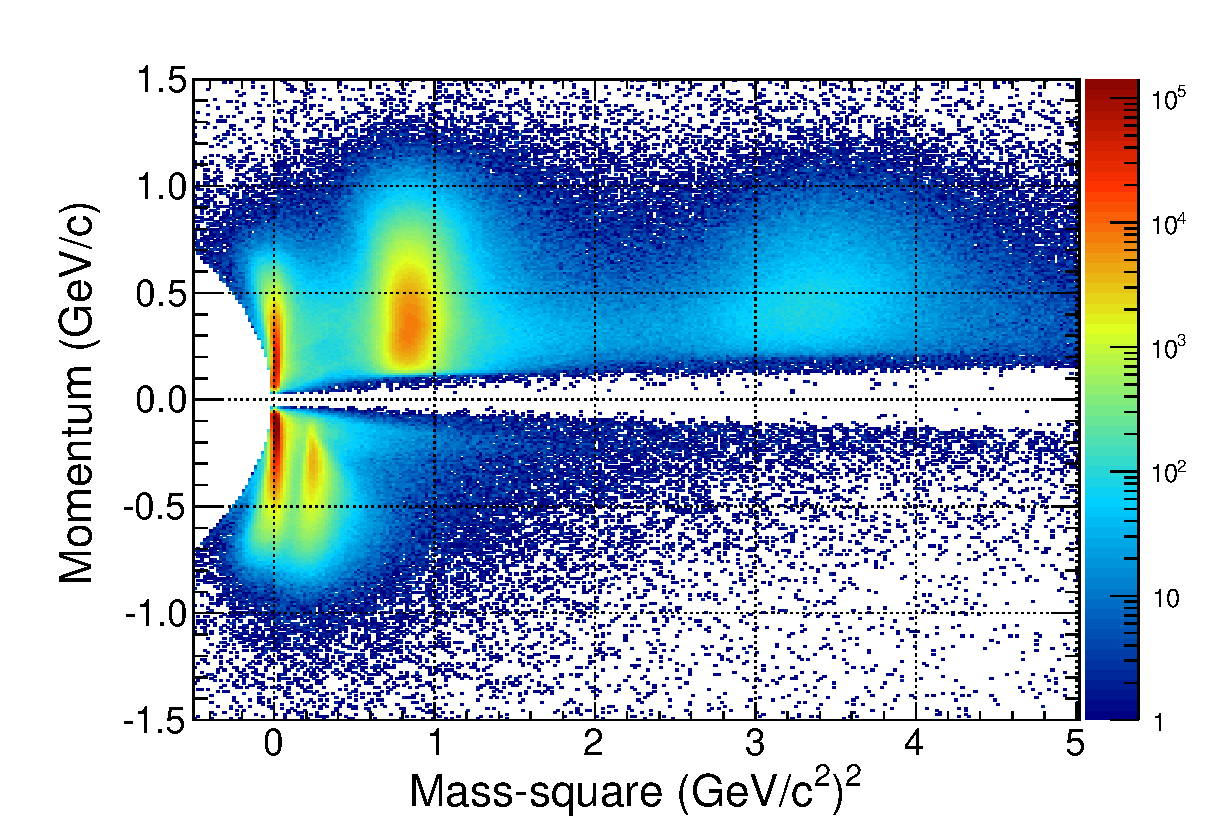
\includegraphics[width=12cm]{./fig/cdcpid2d.eps}
\caption[Two-dimentional PID plot for the CDS particle]{PID plot for the CDS particle. $\pi^+$, protons and deuterons are clearly separated in the positive momentum side, while $\pi^-$ and $K^-$ are in the negative side.}
\label{fig-cdspid2d}
\end{center}
\end{figure}  

\begin{figure}[]
\begin{center}
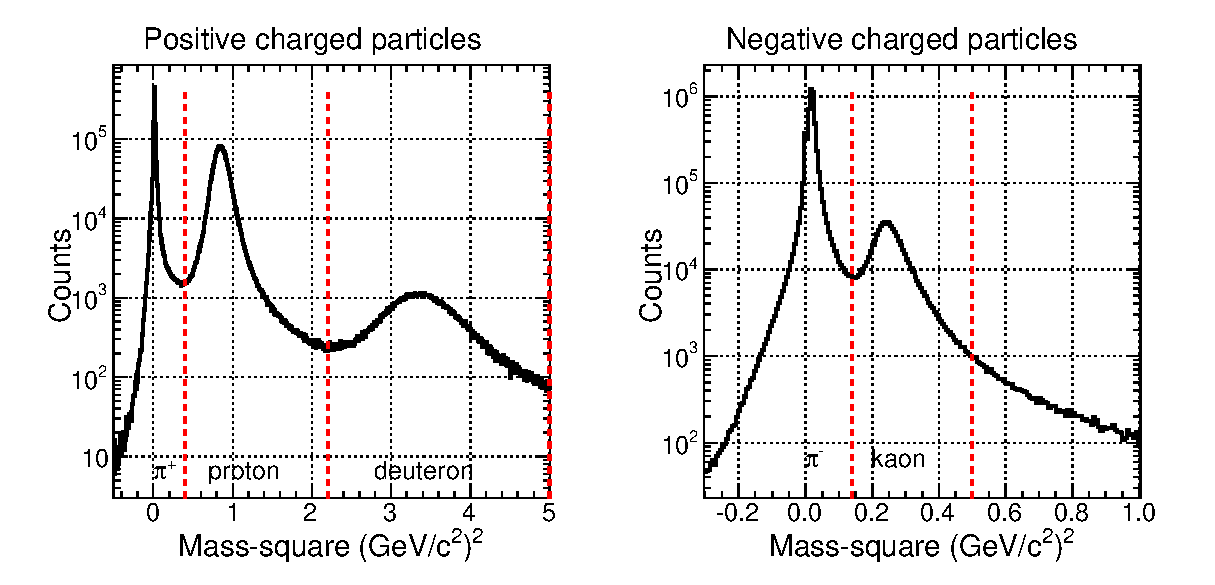
\includegraphics[width=\columnwidth]{./fig/cdcpid1d.eps}
\caption[Mass-square distributions of the CDS particles.]{Mass-square distributions for (left) positive and (right) negative charged particles in the CDS. Particle identification is roughly done with red dotted lines. }
\label{fig-cdspid1d}
\end{center}
\end{figure}  

\subsection{Fine corrections}\label{sec-cdsfinetune}
Following two corrections on the CDC drift time were applied to minimize systematic effects caused by different particle species and the momenta.
\subsubsection{Re-timing of the CDC drift times}
Since the TDC start timing was defined by the T0 timing, the TDC data of the CDC contained the drift time and flight time between T0 and the CDC cell. To extract the drift time, we calculated the flight time by using the helical trajectory, the associated CDH-hit timing, and the velocity calculated in Eq. \ref{eq-cdsbeta}.
\subsubsection{Time-walk effect on the CDC drift times}
A time-walk effect is well known for photon sensors and collected by using the correlation of the integral charge or the pulse height. % as explain in Sec. \ref{}. 
A similar effect should exist in a drift chamber. Although we took only timing information, a pulse height of a CDC signal should be correlated with an evaluated velocity $\beta_{CDC}$. Figure \ref{fig-cdcslew} shows clear correlation between the $1/\beta^2_{CDC}$ and the residual converted to a time scale. This correlation was compensated by fitting with a function $p_0 + p_1x +p_2x^2+ p_3\exp(p_4x)$ as shown in Fig. \ref{fig-cdcslew}. 
\begin{figure}[]
\begin{center}
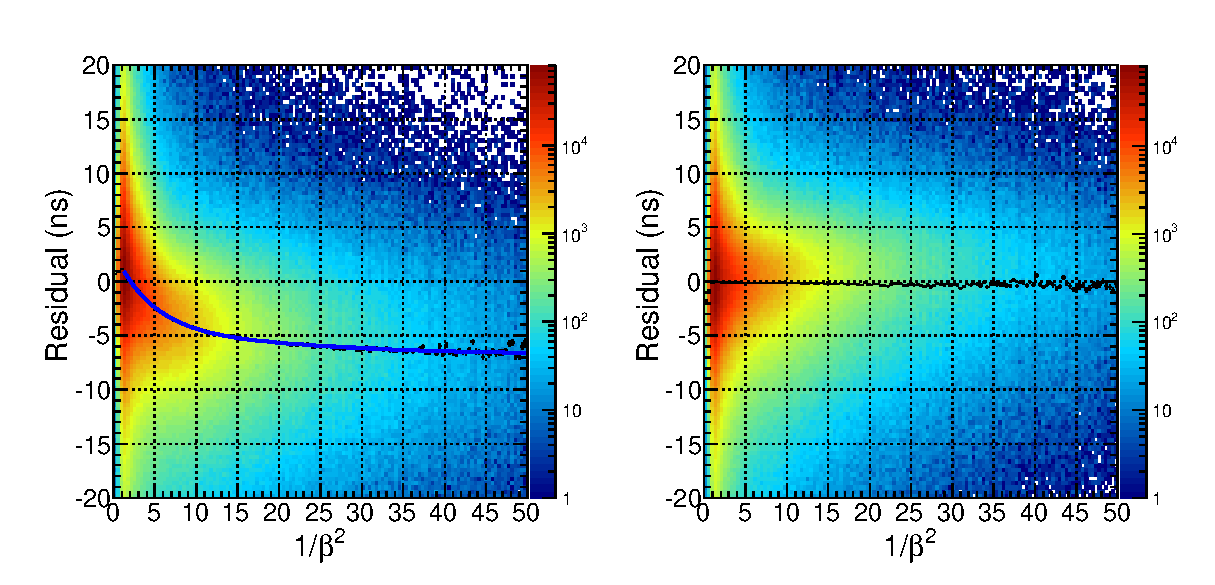
\includegraphics[width=\columnwidth]{./fig/cdcslew.eps}
\caption[Correlation between the 1/$\beta^2$ and the residual of the CDC track]{Correlation between the 1/$\beta^2$ and the residual of the CDC track, (left) before and (right) after fine corrections.}
\label{fig-cdcslew}
\end{center}
\end{figure}  


\subsection{CDS performance}
\subsubsection{Spatial resolution of planes\label{sec-cdcposres}}
Figure \ref{fig-cdcresid} shows the typical residuals. The residuals are compared with those obtained by a Monte-Carlo simulation assuming various spatial resolutions. From the comparison, the spatial resolution in the experimental data was evaluated to be $\sim$180 $\mu$m. This value was used in the Monte-Carlo simulation in this thesis.

As for the systematic differences by the particle species, typical residual distributions are compared in Fig. \ref{fig-cdcresidpikp}. No significant differences were observed.
\begin{figure}[]
\begin{center}
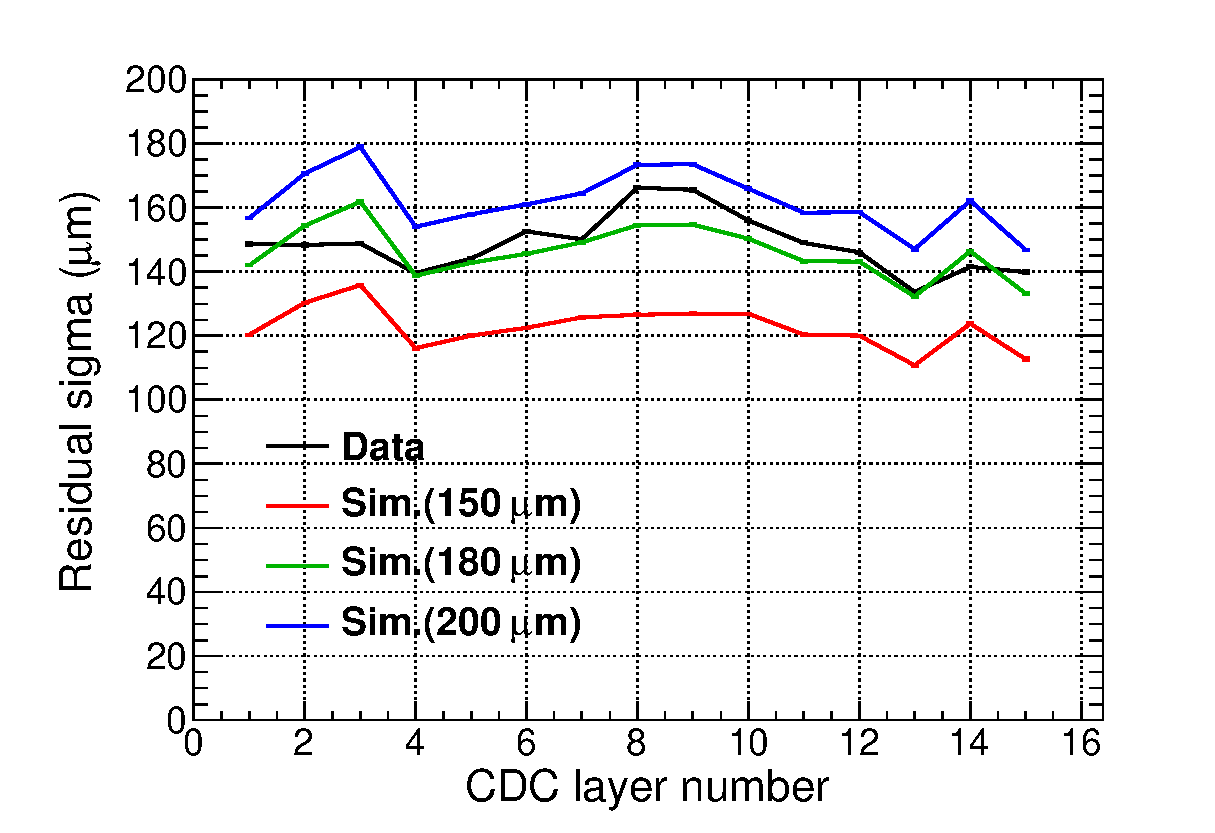
\includegraphics[width=12cm]{./fig/cdcresid.eps}
\caption[Residual distributions of the CDC.]{Comparison of the residual distributions of the CDC between the data and the simulation. The simulation with an intrinsic spatial resolution of 180 $\mu$m agrees with the data.}
\label{fig-cdcresid}
\end{center}
\end{figure}  

\begin{figure}[]
\begin{center}
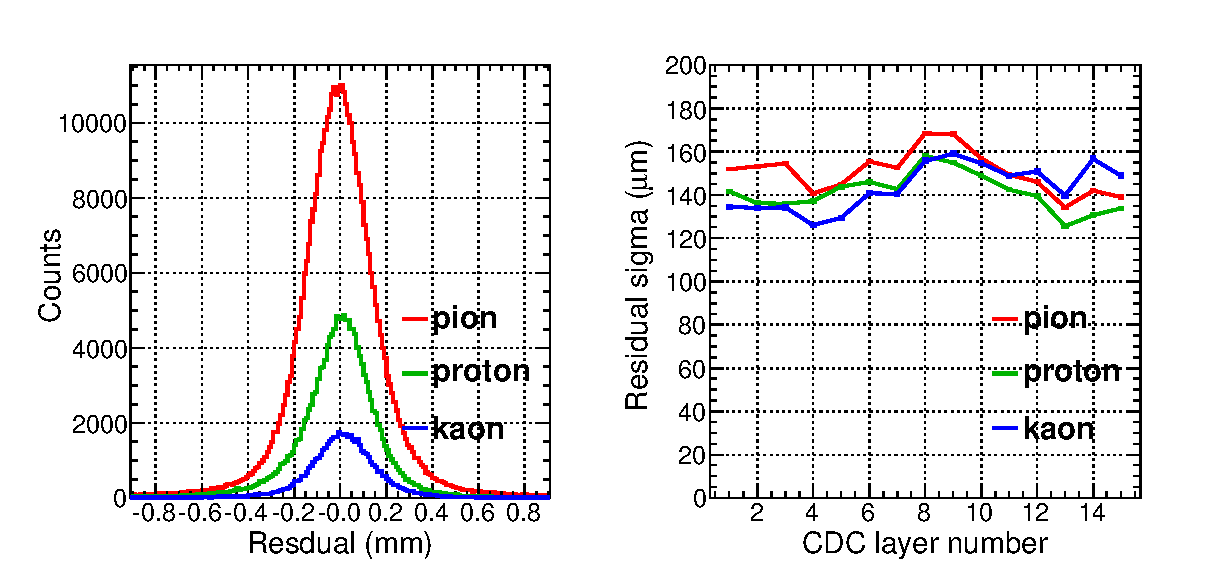
\includegraphics[width=\columnwidth]{./fig/cdcresidpikp.eps}
\caption[Particle dependences of the CDC performances.]{Particle dependences of (left) the shape of the residual distributions and (right) the residuals as a function of the layer number.}
\label{fig-cdcresidpikp}
\end{center}
\end{figure}  

\subsubsection{Momentum resolution}
A transverse momentum resolution for the CDC track was evaluated by the Monte Calro simulation with the spatial resolution as derived above. Figure \ref{fig-cdcsimres} shows the resolutions for pions, kaons and protons.
\if0 Their momentum dependences are expressed as,
\begin{eqnarray*}
\left(\frac{\delta p_t}{p_t}\right) &=& a \cdot p_t + \frac{b}{p_t-c}+d \\
\end{eqnarray*}
where a, b, c, and d are parameters. The obtained parameters are summarized in Table \ref{tab-pikpres} for each particle species. %These were used for particle identification as described in Sec. \ref{sec-cdcpid}.
\fi
\begin{figure}[]
\begin{center}
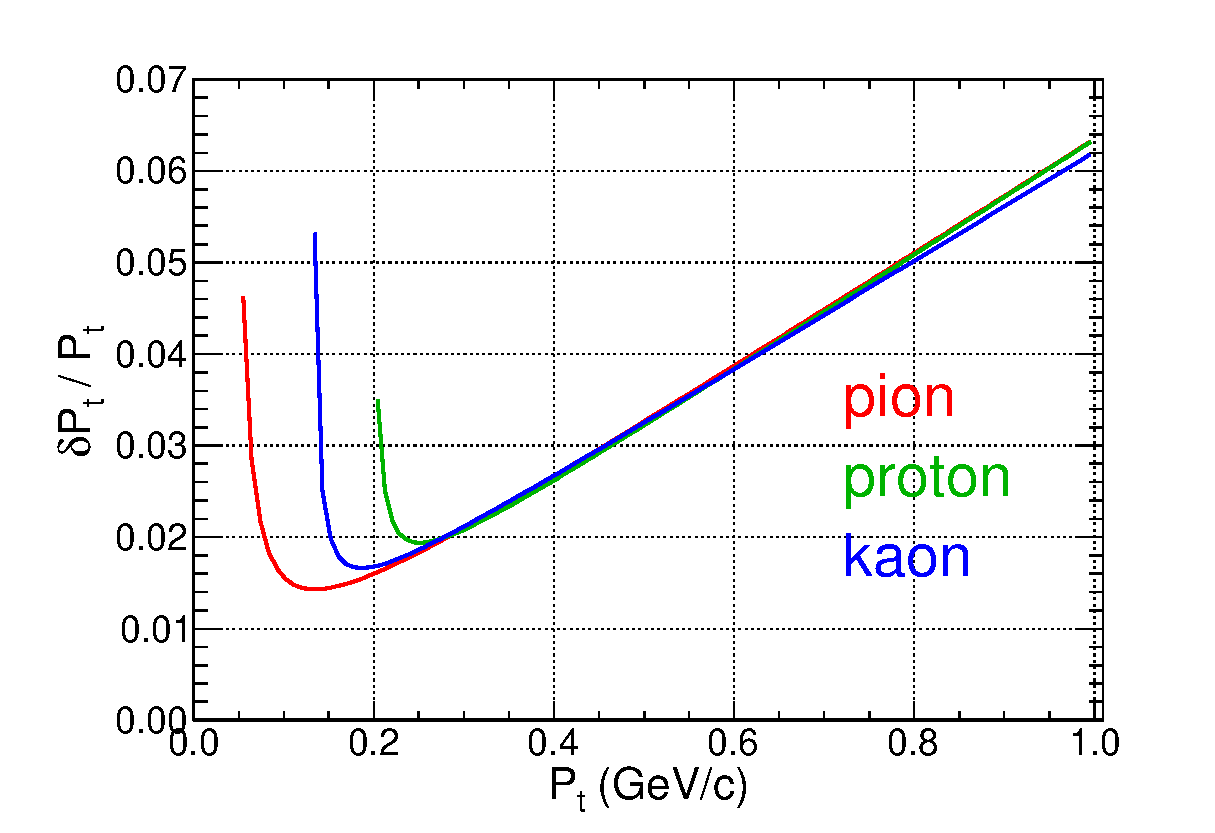
\includegraphics[width=12cm]{./fig/cdcsimres.eps}
\caption{The simulated $p_t$ resolution of the CDC single track for each particle species.}% The points are simulated data and the solid curves are the fit.}
\label{fig-cdcsimres}
\end{center}
\end{figure}  

\if0
\begin{table}[]
\caption{Parameters of the $p_T$ resolutions for each particle species.}
\begin{center}
\begin{tabular}{l|cccc} 
\hline\hline				
particle	&	a		&	b		&	c		&	d		\\
\hline													
$\pi$	&	6.29	$\times 10^{-2}$	&	5.38	$\times 10^{-4}$	&	4.22	$\times 10^{-2}$	&	1.04	$\times 10^{-5}$	\\
kaon	&	5.97	$\times 10^{-2}$	&	1.87	$\times 10^{-4}$	&	1.30	$\times 10^{-1}$	&	2.17	$\times 10^{-3}$	\\
proton	&	6.32	$\times 10^{-2}$	&	2.00	$\times 10^{-4}$	&	1.95	$\times 10^{-1}$	&	-5.62	$\times 10^{-5}$	\\
\hline\hline												
\end{tabular}
\end{center}
\label{tab-pikpres}
\end{table}%
\fi

\subsubsection{CDC tracking efficiency \label{sec-cdceff}}
Tracking efficiencies of CDC were evaluated by using two data samples; one was the cosmic-ray data obtained in the off-spill duration, and the other was the physics data, i.e., secondary charged particles from kaon-induced reactions.

For the cosmic-ray data, we selected events with two separated hits on both the IH and the CDH, which should contains two CDC tracks generated by one cosmic-ray. These event samples are expected to be clean enough since they are almost free from accidentals and neutral particles. For the cosmic data, we obtained the tracking efficiency of 97.8 $\pm$ 0.2\%. The error was evaluated from the fluctuations during the experimental period. 

In contrast, the kaon-induced data is expected to contain much more backgrounds. To reduce the background contributions from beam-pileup events and neutral particles, strict cuts were applied as follows:
\begin{enumerate}
\item The beam was required to be a single particle and hit on the target.
\item Select single-CDH-hit events with more than 5 MeV$ee$ (electron equivalent) energy deposits on both CDH PMTs. Timing selection was applied to exclude $\gamma$-ray events.
\item The azimuthal-angle difference between the CDH and the IH hit-segments was required to be less than 20$^\circ$.
\end{enumerate}
With this event selection, the tracking efficiency was obtained to be 94.0 $\pm$ 0.5\%. The error was evaluated in the same way as the cosmic-ray data.

Although there is some discrepancy in the obtained efficiencies, the two data-samples would give extreme cases of the measurement conditions. Therefore, we adopted the mean values of 96 $\pm$ 2\% in the current analysis, where the error was evaluated from the deviation.
%The stability of the CDC tracking efficiency is plotted in Fig. \ref{}.
\subsubsection{Vertex resolution\label{sec-cdsvres}}

The vertex resolution was evaluated with the kaon-induced tracks. The vertex was reconstructed for every CDC track with the beam track. As for the resolution in the $xy$ plane, the reconstructed vertices around $x(y)$=0, $z$=0 cm were selected and the $y(x)$ position distribution was checked.  In Fig. \ref{fig-cdcposres}(left) two clear peaks which correspond to the target cell with 0.3 mm thickness are observed. As a result of Gaussian fitting of these peaks, the $xy$ vertex resolution was evaluated to be $\sim$1 mm, which was almost solely determined by the resolution of the beam track.
Figure \ref{fig-cdcposres}(right) shows $z$ vertex distribution with $x^2+y^2<2$ cm$^2$. The largest peak around $-$16 cm corresponds to the DEF. By fitting the DEF peak and considering the DEF thickness of 3 mm, the $z$ vertex resolution was evaluated to be $\sim$7 mm. Both $xy$ and $z$ vertex resolutions are consistent with those obtained by the simulation.
\begin{figure}[]
\begin{center}
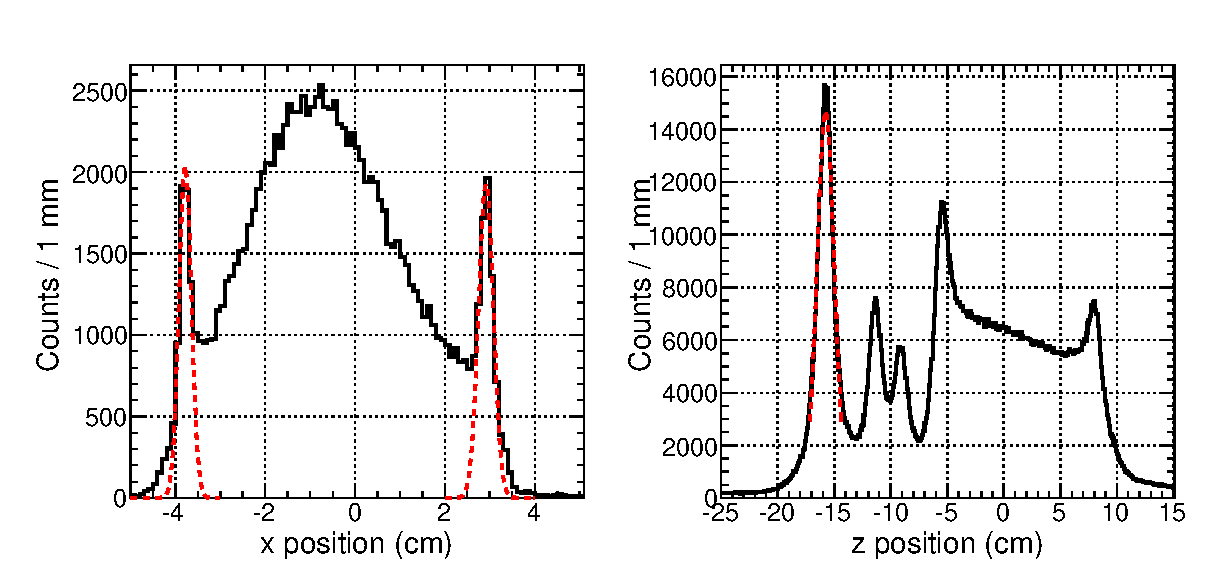
\includegraphics[width=\columnwidth]{./fig/cdcxyres.eps}
\caption[$x$ and $z$ vertex position distributions.]{(left) Reconstructed $x$ vertex position distribution around $y$=$z$=0 cm. The two distinct peaks correspond to the target cell. (right) Reconstructed $z$ vertex position distribution. The most prominent peak at around $z=-$16 cm is the position of the DEF. The red dotted lines are the Gaussian fitting results to evaluate the vertex resolutions.}
\label{fig-cdcposres}
\end{center}
\end{figure}  

\subsection{Fiducial volume selection\label{sec-fiducial}}
The vertex distribution in the $zy$ plane and the $zx$ plane are shown in Fig. \ref{fig-cdcvertex}. The target cell is clearly identified in addition to the DEF, the vacuum vessel, the thermal radiation shield, and the $^3$He transfer pipes. The fiducial volume of the $^3$He target is defined as the blue boxes in Fig. \ref{fig-cdcvertex}, whose size is 30 mm radius $\times$ 100 mm length. The fiducial volume is apart from the beryllium cylinder of the target cell by more than 3 times the $xy$ resolution to reduce contaminations from other materials. The $z$ length and position of the fiducial volume is defined by that of the beryllium cylinder to avoid material complexity in other parts of the cell.  
\begin{figure}[]
\begin{center}
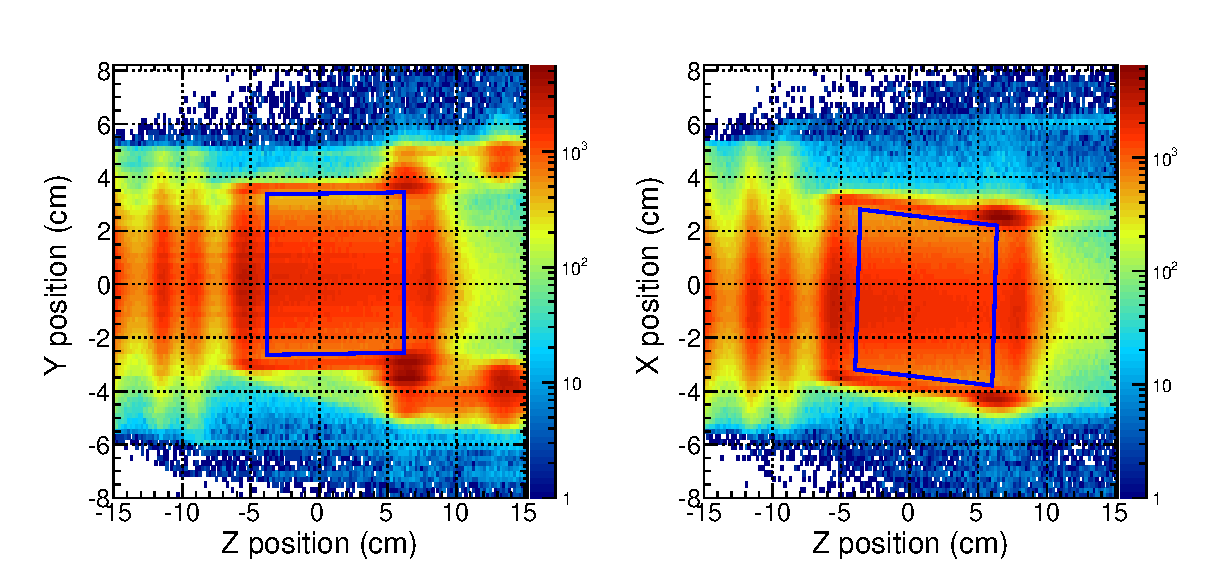
\includegraphics[width=\columnwidth]{./fig/cdcvertex.eps}
\caption[Definition of the fiducial volume.]{Reconstructed vertex distribution in (left) the $zy$ and (right) the $zx$ planes. The fiducial volume is defined as the blue boxes. }
\label{fig-cdcvertex}
\end{center}
\end{figure}  

\subsection{$K^0_s$ and $\Lambda$ reconstruction\label{sec-cdck0}}
To confirm the spectrometer performance of the CDS,  the invariant masses of $\pi^+\pi^-$ pairs and $p\pi^-$ pairs were reconstructed as shown in Fig. \ref{fig-cdck0}  and Fig. \ref{fig-cdclambda}, respectively. Clear peaks of $K^0_s\to\pi^+\pi^-$ and $\Lambda\to\pi^-p$ decays were obtained in the invariant mass distributions. Their positions are consistent with PDG values within 1 MeV/$c^2$ precision after an adjustment of the field strength of the solenoid magnet described below. %The peak widths are also consistent with those obtained by the simulation.
\begin{figure}[]
\begin{center}
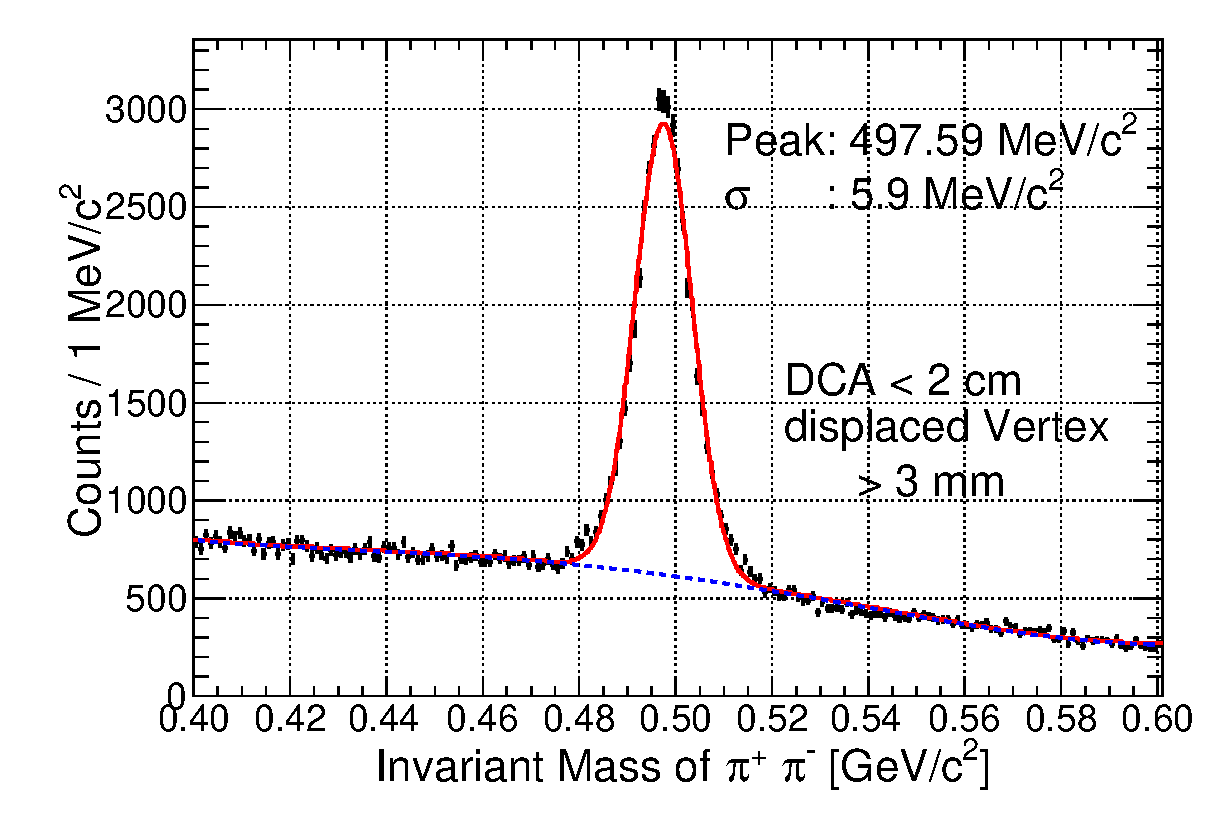
\includegraphics[width=10cm]{./fig/cdck0.eps}
\caption[Invariant mass distribution of $\pi^+\pi^-$ pairs reconstructed with the CDS. ]{Invariant mass distribution of $\pi^+\pi^-$ pairs reconstructed with the CDS. The $K^0_s$ peak was fitted with a Gaussian and a third-order polynomial background. The red solid curve and the blue dotted curve show the fitting result and background contribution, respectively.}% The vertical dotted lines show the $K^0_s$ selection region in the later analysis. }
\label{fig-cdck0}
\end{center}
\end{figure}  

\begin{figure}[]
\begin{center}
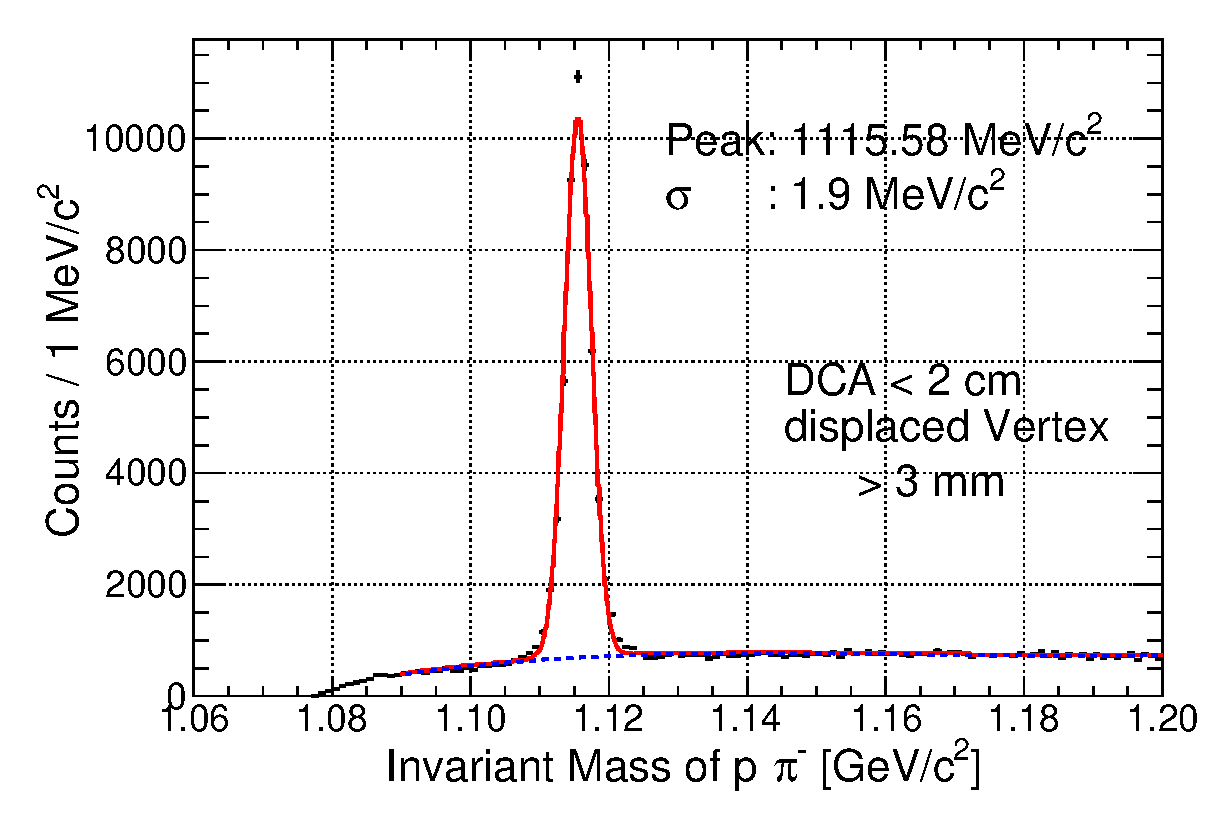
\includegraphics[width=10cm]{./fig/cdclambda.eps}
\caption[Invariant mass distribution of $p\pi^-$ pairs reconstructed with the CDS. ]{Invariant mass distribution of $p\pi^-$ pairs reconstructed with the CDS. The $\Lambda$ peak was fitted with a Gaussian and a third-order polynomial background. The red solid curve and the blue dotted curve show the fitting result and background contribution, respectively.}% The vertical dotted lines show the $\Lambda$ selection region in the later analysis.}
\label{fig-cdclambda}
\end{center}
\end{figure}  

\subsubsection{Adjustment of the CDS field strength}
Since we were not able to measure the magnetic field strength of the CDS in the final setup, the value should be adjusted by using the data. $K^0_s$ and $\Lambda$ peaks are good calibration source for this purpose. The field strength was changed a little so that the both peak positions were consistent to the PDG values with in 1 MeV/$c^2$ as shown in Fig.~\ref{fig-cdcfield}. We found the requirement is satisfied when the magnetic field is 
\begin{eqnarray}
0.715   \pm 0.002\ {\rm T}, 
\end{eqnarray}
where the error was assumed to be symmetric.

\begin{figure}[]
\begin{center}
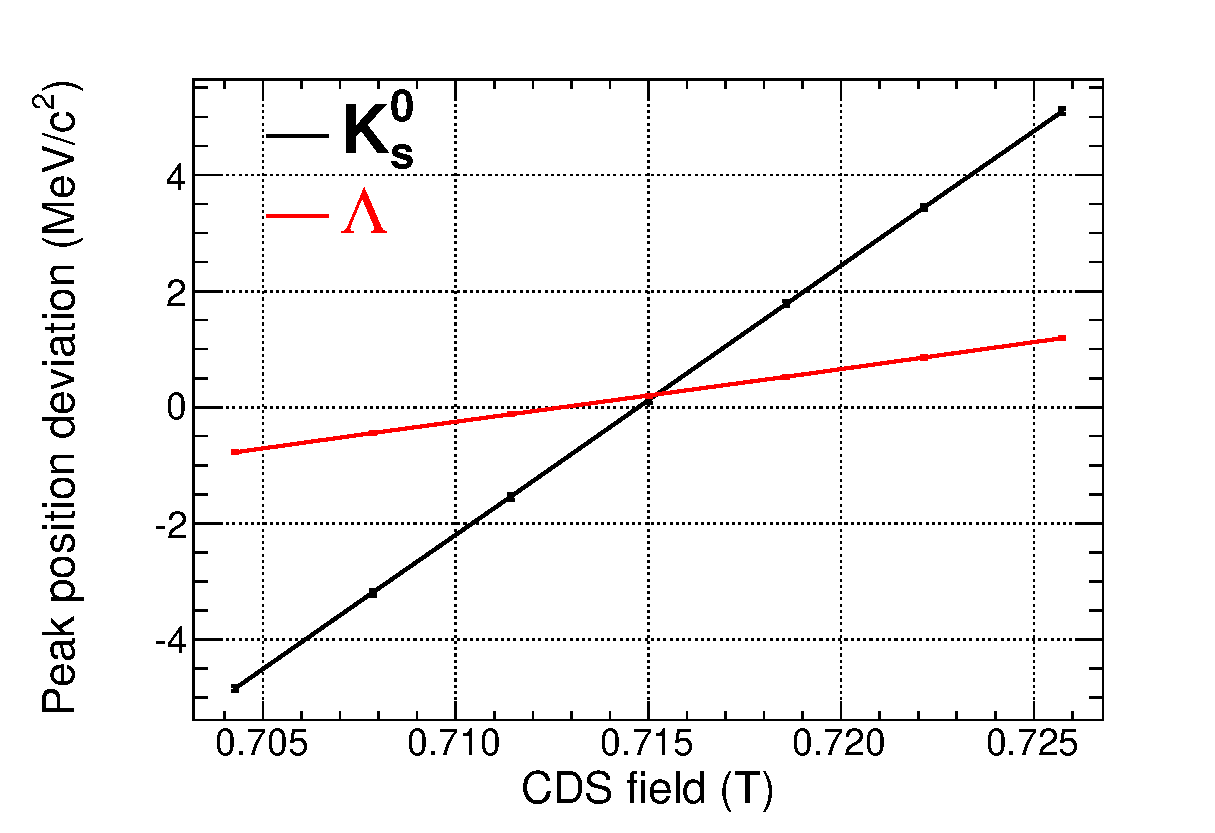
\includegraphics[width=10cm]{./fig/cdcfield.eps}
\caption[Optimization of the CDS field strength.]{The correlation between the peak position deviations of $K^0_s$ and $\Lambda$ from the PDG values and the CDS field. The center value of the CDS field is set to be 0.715T.  }
\label{fig-cdcfield}
\end{center}
\end{figure} 

\if0 % appendix??
\subsection{Topological selection}
In the CDS analysis, we sometimes applied topological selection to improve the signal-to-noise ratio. 
\subsubsection{CDC single track analysis}
If we analyze single track of the CDC, there is only one parameter $D_{CA}$ (Fig. \ref{}) to define the property of the topology. The typical $D_{CA}$ distribution is shown in Fig. \ref{}.
\subsubsection{CDC two track analysis}
As shown in Fig. \ref{}, three parameters $D_{CA}^{CDC}$, $D_{CA}^{beam}$ and $D_{vertex}$ appear in two track analysis. Their typical distributions are show in Fig. \ref{} for $K^0_s$
\fi